\documentclass[11pt,a4paper]{article}

\usepackage[margin=1in]{geometry}
\usepackage{amsmath,amssymb,amsthm}
\usepackage{mathtools}
\usepackage{hyperref}
\usepackage{booktabs}
\usepackage{longtable}
\usepackage{array}
\usepackage{tikz}
\usetikzlibrary{arrows.meta,positioning}
\usepackage{enumitem}

\hypersetup{
  colorlinks=true,
  linkcolor=blue!50!black,
  citecolor=blue!50!black,
  urlcolor=blue!60!black
}

\newtheorem{conjecture}{Conjecture}
\newtheorem{problem}{Open Problem}
\theoremstyle{definition}
\newtheorem{definition}[conjecture]{Definition}
\theoremstyle{remark}
\newtheorem{remark}[conjecture]{Remark}

\newcommand{\PSLZ}{\mathrm{PSL}_2(\mathbb{Z})}
\newcommand{\PCF}{\mathrm{PCF}}
\newcommand{\Q}{\mathbb{Q}}
\newcommand{\Z}{\mathbb{Z}}
\newcommand{\R}{\mathbb{R}}
\newcommand{\C}{\mathbb{C}}
\newcommand{\OO}{\mathcal{O}}

\title{An Arithmetic Stratification of Polynomial Continued Fractions:\\
       Program Statement of the SIARC Series}
\author{papanokechi}
\date{April 2026}

\begin{document}
\maketitle

\begin{abstract}
This paper is a \emph{program statement}, not a results paper. It articulates
the logical structure of the SIARC series: a body of $6$--$8$ companion papers
that together propose an arithmetic stratification of polynomial continued
fractions (PCFs) organized by the underlying uniformizing Fuchsian group and
by an obstruction tier. We state the four-tier hierarchy
(Algebraic / Transcendental / Trans-stratum / Barrier), present the
Trans-stratum two-class conjecture (Class A at $a_2/b_1^2 = -2/9$,
Class B at $a_2/b_1^2 = +1/4$) in precise form, list the open problems
that anchor the program, and tabulate the role and current status of each
companion paper. \emph{No proofs are reproduced here}; every nontrivial
claim is either stated as a conjecture or remarked upon with a pointer to
the appropriate companion paper, cited by Zenodo DOI where available. The
purpose of this document is to provide a stable, citable scope-anchor for
the program and to fix unified notation across the series.
\end{abstract}

\tableofcontents

\section{Introduction and Motivation}
\label{sec:intro}

A \emph{polynomial continued fraction} (PCF) is a formal continued fraction
\begin{equation}
  \label{eq:pcf-def}
  K(x) \;=\; b_0(x) + \cfrac{a_1(x)}{b_1(x) + \cfrac{a_2(x)}{b_2(x) + \cfrac{a_3(x)}{b_3(x) + \ddots}}}
\end{equation}
in which the partial numerators $a_n(x)$ and partial denominators $b_n(x)$
are fixed polynomials in $x$ with integer (or rational) coefficients, evaluated
at a fixed integer $x \in \Z_{\geq 1}$. The classical Ramanujan and
Rogers--Ramanujan continued fractions, the Stern--Brocot expansions of
quadratic irrationals, and the Apéry-style recurrences for $\zeta(2)$ and
$\zeta(3)$ are all PCFs in this sense. A central problem, going back to
Stieltjes and revisited in the modern era by Lagarias, Borwein, and others,
is to determine the \emph{arithmetic nature} of the limit of \eqref{eq:pcf-def}:
when is it rational, when is it algebraic, when is it transcendental, and
when does it fail to converge to a number that admits any such classification?

The SIARC program proposes that this arithmetic question is not
homogeneous. PCFs admit a natural \emph{stratification} indexed by
(i) the uniformizing Fuchsian group of the associated monodromy
representation, and (ii) an obstruction tier that records how far the
limit lies from being algebraic over $\Q$. This stratification organizes
otherwise unrelated empirical phenomena --- the appearance of $-2/9$
exponents in degree-$(2,1)$ families, the Painlevé connection in
degree-$(3,1)$ families, the failure of the Mahler criterion at
specific lattice points --- into a single arithmetic picture.

\paragraph{Goal of the program.}
The SIARC program aims to define, for each Fuchsian group $\Gamma$ that
arises as a uniformizer of a PCF family, a four-tier arithmetic
stratification (\S\ref{sec:tiers}), to verify the stratification on the
$\PSLZ$ case completely (companion paper \#14), and to extend it
conjecturally to the remaining classical groups via the Trans-Stratum
Conjecture (\S\ref{sec:t2b}) and the open problems of \S\ref{sec:open}.

\section{The Four-Tier Hierarchy}
\label{sec:tiers}

We summarize the tier definitions. Full proofs of the classification
theorem are deferred to the $\PSLZ$ paper; see Remark~\ref{rem:tiers-source}.

\begin{definition}[Tier T0: Algebraic]
A PCF family $\{K(x)\}_{x \in S}$ lies in tier T0 over an arithmetic set
$S \subseteq \Z_{\geq 1}$ if $K(x)$ is algebraic over $\Q$ for every
$x \in S$, and the algebraic degree is uniformly bounded as $x$ varies in $S$.
\end{definition}

\begin{definition}[Tier T1: Transcendental]
A PCF family lies in tier T1 if $K(x)$ is transcendental for every $x \in S$,
\emph{and} a Mahler-type or Nesterenko-type criterion certifies the
transcendence uniformly in $x$.
\end{definition}

\begin{definition}[Tier T2: Trans-stratum]
A PCF family lies in tier T2 if its irrationality measure $\mu(K(x))$
satisfies an asymptotic
\[
   \mu(K(x)) \;=\; 2 + \frac{c}{\log x} + o\!\left(\frac{1}{\log x}\right),
   \qquad x \to \infty,
\]
for an explicit rational constant $c$ (the \emph{trans-stratum exponent})
that depends only on the polynomial degrees $(\deg a, \deg b)$ and the
Fuchsian group $\Gamma$. The trans-stratum is therefore not a transcendence
statement, but a statement about the rate at which transcendence is
approached.
\end{definition}

\begin{definition}[Tier T3: Barrier]
A PCF family lies in tier T3 if the Fuchsian uniformization itself
degenerates: either $\Gamma$ fails to be of finite covolume, or the
associated $L$-function fails to admit analytic continuation to the
required half-plane. T3 families are inaccessible to the methods of T0--T2
and serve as the negative boundary of the program.
\end{definition}

\begin{remark}[Translation to the obstruction hierarchy of \#14]
\label{rem:tier-translation}
The companion paper~\#14 introduces a parallel four-tier
\emph{obstruction} hierarchy $O_0,\dots,O_3$ measuring the
distance from the modular sector $X(1)$. The two
hierarchies do not coincide. We have the inclusions
$O_0 \subseteq T_0 \cup T_2$, $O_1 \subseteq T_2$,
$O_2 \subseteq T_2$, $O_3 \subseteq T_3$, but in general
neither family of tiers refines the other. We use $T_0,\dots,T_3$
exclusively for the arithmetic hierarchy of this paper, and
$O_0,\dots,O_3$ for the obstruction hierarchy of~\#14.
\end{remark}

\begin{remark}[Source of the classification]
\label{rem:tiers-source}
A full classification theorem stating that every $\PSLZ$-uniformized
PCF family lies in exactly one of T0, T1, T2, T3 --- and that the
tier is computable from $(\deg a, \deg b)$ and the leading coefficients
--- is the main theorem of companion paper \#14. We do not reproduce
either the statement in full generality or the proof here. See the
companion paper table in \S\ref{sec:companions}.
\end{remark}

\section{Logical Structure of the Program}
\label{sec:structure}

\subsection{Companion papers and dependency graph}

Figure~\ref{fig:depgraph} shows the dependency structure of the
program. The $\PSLZ$ classification (\#14) is foundational; the
Trans-Stratum paper (T2B) sharpens its T2 stratum; the Painlevé
paper (P08) connects T2 to nonlinear special functions; the
remaining papers extend the stratification to non-$\PSLZ$
Fuchsian groups.

\begin{figure}[h]
\centering
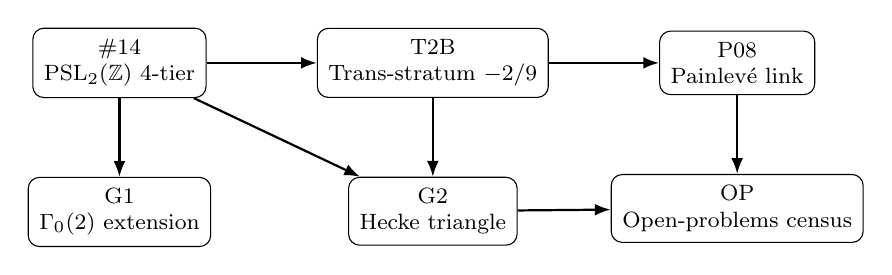
\begin{tikzpicture}[
  node distance=10mm and 14mm,
  every node/.style={draw, rounded corners, align=center,
                     font=\footnotesize, inner sep=4pt},
  arr/.style={-{Latex[length=2mm]}, thick}
]
\node (p14) {\#14\\ $\PSLZ$ 4-tier};
\node (t2b) [right=of p14] {T2B\\ Trans-stratum $-2/9$};
\node (p08) [right=of t2b] {P08\\ Painlevé link};
\node (g1)  [below=of p14] {G1\\ $\Gamma_0(2)$ extension};
\node (g2)  [below=of t2b] {G2\\ Hecke triangle};
\node (op)  [below=of p08] {OP\\ Open-problems census};

\draw[arr] (p14) -- (t2b);
\draw[arr] (t2b) -- (p08);
\draw[arr] (p14) -- (g1);
\draw[arr] (p14) -- (g2);
\draw[arr] (t2b) -- (g2);
\draw[arr] (p08) -- (op);
\draw[arr] (g2)  -- (op);
\end{tikzpicture}
\caption{Dependency graph of the SIARC companion papers. Arrows
denote ``logical prerequisite''; the umbrella paper (this document)
sits above all nodes and provides the unified notation.}
\label{fig:depgraph}
\end{figure}

\subsection{Unified notation}

Across the series we adopt the following conventions. Companion papers
that predate this umbrella may use slightly different notation locally;
the table below is the canonical reference.

\begin{center}
\begin{tabular}{@{}lll@{}}
\toprule
Symbol & Meaning & Convention \\
\midrule
$x$ & PCF variable & integer, $x \geq 1$ \\
$a_n(x), b_n(x)$ & partial num./denom.\ polynomials & $\Z[x]$ \\
$(d_a, d_b)$ & degree pair & $d_a = \deg a_n$, $d_b = \deg b_n$ \\
$\Gamma$ & uniformizing Fuchsian group & subgroup of $\PSLZ$ unless stated \\
$K(x)$ & limit of the PCF at $x$ & in $\R \cup \{\infty\}$ \\
$\mu(\alpha)$ & irrationality measure of $\alpha$ & $\mu \geq 2$ for irrationals \\
$c_{\Gamma,(d_a,d_b)}$ & trans-stratum exponent & rational, depends on $\Gamma$ and degrees \\
T0--T3 & tiers & as in \S\ref{sec:tiers} \\
\bottomrule
\end{tabular}
\end{center}

\noindent
\textbf{Degree convention.} Throughout the series, ``degree-$(d_a, d_b)$''
refers to the \emph{generic} polynomial degrees of $a_n$ and $b_n$ as
functions of the index $n$ in the underlying recurrence, not as
functions of $x$. A degree-$(2,1)$ family is therefore one in which
the numerator polynomial grows quadratically in $n$ and the denominator
grows linearly in $n$.

\section{The Trans-Stratum Conjecture}
\label{sec:t2b}

The single most distinctive empirical phenomenon of the program is
the persistent appearance of the rational exponent $-2/9$ in the
trans-stratum of degree-$(2,1)$ families uniformized by $\PSLZ$.

\begin{conjecture}[Trans-stratum two-class conjecture]
\label{conj:t2b}
Let $\{K(x)\}$ be a PCF family of generic degree $(2,1)$
uniformized by $\PSLZ$, satisfying the regularity conditions
of companion paper~T2B.  Then $K(x)$ lies in tier T2 and falls
into exactly one of two classes, distinguished by the
structural ratio $\rho := a_2/b_1^2$:
\begin{itemize}
  \item Class A ($\rho = -2/9$): trans-stratum exponent
        $c_{\PSLZ,(2,1),A} = -2/9$ (T2B Theorem~2,
        conditional on $S_{12}\neq 0$);
  \item Class B ($\rho = +1/4$): limits lie in
        $\mathbb{Q}(\pi)$ (T2B Theorem~3); the Pure-regime
        subclass satisfies the stronger $\mathbb{Q}\cdot\pi^{-1}$
        (T2B Cor.~classB-pi).
\end{itemize}
Equivalently (T2B Completeness Conjecture): the degree-$(2,1)$
Trans-stratum is exactly $\mathcal{T}_A \sqcup \mathcal{T}_B$,
with no third class.
\end{conjecture}

\begin{remark}[Pre-revision form]
\label{rem:t2b-prerev}
The version of this conjecture in UMB v1 (Zenodo
\href{https://doi.org/10.5281/zenodo.19885550}{10.5281/zenodo.19885550})
stated only the Class A clause.  The current form incorporates the
Class B census of companion paper~T2B (16 canonical families,
height $\leq 100$).  No previously asserted Class A claim is revoked;
the change is purely additive.
\end{remark}

\begin{remark}[Empirical basis]
\label{rem:empirical}
A computational census reported in companion paper~T2B
(Zenodo concept DOI \href{https://doi.org/10.5281/zenodo.19783311}{10.5281/zenodo.19783311})
covers approximately $150{,}000$ degree-$(2,1)$ families generated
under the regularity conditions of that paper. Across the entire
census, no counterexample to Conjecture~\ref{conj:t2b} has been
observed; the empirical fit to the predicted $-2/9$ slope is consistent
with the reported numerical precision. We do not reproduce the
empirical methodology, the regularity conditions, or any proof
attempt in this document; all such material lives in T2B.
\end{remark}

\begin{remark}[Why $-2/9$?]
The value $-2/9$ arises in companion paper~T2B via the
indicial exponents $\{1/3, 2/3\}$ of the associated
three-term recurrence at infinity: the ratio $a_2/b_1^2$
is determined by requiring the indicial roots to sum to
$1$ and multiply to $2/9$, giving $1/3 + 2/3 = 1$ and
$(1/3)(2/3) = 2/9$. A congruence-subgroup interpretation
of this denominator is speculative and not established;
a rigorous derivation from the monodromy of the
uniformizing group remains the central open problem.
\end{remark}

\begin{remark}[Projective verification of Conjecture~\ref{conj:t2b}, Class A]
\label{rem:projective-verify}
A targeted projective-coordinate sweep
($H = 8$, $b_1 \in \{3, 6, \ldots, 30\}$ subject to $3 \mid b_1$,
$48{,}552$ primitive 5-tuples
$(a_2, a_1, a_0, b_1, b_0)$ satisfying $9 a_2 + 2 b_1^2 = 0$,
$\gcd = 1$, $b_1 > 0$; $43{,}915$ distinct-$L$ families;
stratified random sample of $400$ groups, $40$ per $b_1$ bucket)
confirms the Class A clause of Conjecture~\ref{conj:t2b}
empirically: $387/400$ sampled families are Trans, with
$0$ Log, $0$ Alg, $13$ rational, and $0$ phantom hits
under PSLQ at \texttt{dps}$=400$, $\mathrm{tol} = 10^{-50}$,
basis $\{1, \pi, \pi^2, \log 2, \zeta(2), \zeta(3),
\sqrt{2}, \sqrt{3}, \sqrt{5}, e, \gamma, \log 3,
\pi \log 2, \pi^2, \pi^3\}$, with mandatory rejection of any
relation whose $L$-coefficient vanishes. The smallest
witness is
$(a_2, a_1, a_0, b_1, b_0) = (-2, 0, 1, 3, -1)$ with
$L \approx 0.26057$. An earlier affine-coordinate
enumeration at fixed height $H = 5$
($b_1 \in \{9, 12, 15, 30\}$) found $0$ Trans families;
the discrepancy is a coordinate artefact resolved by passing
to projective normalization with $\gcd = 1$ and $b_1 > 0$,
which admits primitive small-coefficient witnesses
(in particular $b_1 = 3$ with $|a_1|, |a_0|, |b_0| \leq 1$)
that are absent from any fixed-height affine slice.
Every $3 \mid b_1$ bucket in the sample contains at least
$32$ Trans families. Full numerics, classifier source, and
sample data are recorded in
\texttt{sessions/2026-04-30/UMB-RES-EXTEND-PROJ/} of the
SIARC relay bridge repository.
\end{remark}

\section{Open Problems}
\label{sec:open}

We list the principal open problems of the program in rough order of
expected tractability. Each is stated informally; precise formulations
appear in the indicated companion papers.

\begin{problem}[Degree-$(3,1)$ classification]
\label{prob:31}
Establish the four-tier classification for $\PSLZ$-uniformized PCF
families of generic degree $(3,1)$. The asymmetry between numerator and
denominator degrees breaks the symmetric treatment of \#14.
\end{problem}

\begin{problem}[Trans-stratum at $d=2$ for non-$\PSLZ$]
\label{prob:t2-d2-nonpsl}
Determine the trans-stratum exponent $c_{\Gamma,(2,1)}$ for
$\Gamma = \Gamma_0(2)$ and for the Hecke triangle groups $G_q$ with
$q \geq 4$. Is the value $-2/9$ specific to $\PSLZ$, or does it
recur with a $\Gamma$-dependent denominator?
\end{problem}

\begin{problem}[Painlevé connection]
\label{prob:painleve}
Make precise the conjectural correspondence between trans-stratum PCF
families and solutions of Painlevé~VI with monodromy in $\Gamma$.
A pointer-level discussion is given in companion paper~P08; a full
correspondence theorem is open.
\end{problem}

\begin{problem}[Effective T0/T1 boundary]
\label{prob:effective}
Provide an algorithm that, given the polynomials $a_n(x), b_n(x)$ in
exact arithmetic, decides in finite time whether the family lies in
T0 or T1. \#14 establishes the boundary as a set; effectivity is open.
\end{problem}

\begin{problem}[T3 nonemptiness]
\label{prob:t3}
Exhibit an explicit PCF family that provably lies in T3 (not merely
fails to lie in T0--T2 by current methods). Equivalently, exhibit a
PCF whose monodromy group has infinite covolume in a controlled way.
\end{problem}

\begin{problem}[Mahler-Nesterenko gap]
\label{prob:mahler}
For T1 families, identify the precise hypothesis that fails when the
Mahler criterion does not apply and the Nesterenko criterion does.
The empirical gap is small; a structural explanation is missing.
\end{problem}

\begin{problem}[Census completeness]
\label{prob:census}
Extend the empirical census underlying Conjecture~\ref{conj:t2b}
beyond degree-$(2,1)$. A negative result --- a single counterexample
in any degree --- would falsify the Trans-Stratum Conjecture as
stated and force a refinement.
\end{problem}

\section{Companion Papers and Status}
\label{sec:companions}

The table below records the current state of the SIARC series at
the time of this umbrella draft. DOIs marked ``--'' are not yet
issued; DOIs marked ``TBA'' are pending. Statuses are intended to be
updated in revisions of this document.

\begin{center}
\renewcommand{\arraystretch}{1.15}
\begin{longtable}{@{}p{0.08\linewidth} p{0.34\linewidth} p{0.22\linewidth} p{0.28\linewidth}@{}}
\toprule
ID & Title (working) & Venue / status & Zenodo DOI \\
\midrule
\endfirsthead
\toprule
ID & Title (working) & Venue / status & Zenodo DOI \\
\midrule
\endhead
\#14 & Four-tier classification of $\PSLZ$-uniformized PCFs & Submitted; under revision after two desk-rejects on citation hygiene & TBA (post-acceptance) \\
T2B  & Two arithmetic classes of degree-$(2,1)$ Trans-stratum continued fractions: a Birkhoff--Trjitzinsky / Gauss-continued-fraction dichotomy & Preprint on Zenodo (v3.0, 2026-04-30) & \href{https://doi.org/10.5281/zenodo.19915689}{10.5281/zenodo.19915689} \\
P08  & Painlevé~VI and trans-stratum PCFs (pointer paper) & Draft & -- \\
G1   & Extension of the four-tier hierarchy to $\Gamma_0(2)$ & Draft & -- \\
G2   & Trans-stratum exponents for Hecke triangle groups & Outline & -- \\
OP   & Open-problems census for the SIARC program & Outline; partially superseded by \S\ref{sec:open} of this paper & -- \\
UMB  & \emph{This document} (umbrella program statement) & Preprint on Zenodo & \href{https://doi.org/10.5281/zenodo.19885550}{10.5281/zenodo.19885550} \\
\bottomrule
\end{longtable}
\end{center}

\paragraph{Note on proofs.}
By design, no proof from any of the above papers is reproduced in this
document. Where a claim in this document would require proof, it has
been stated as a conjecture, an open problem, or a remark with a pointer
to the responsible companion paper. Readers seeking proofs should
consult the cited companion paper directly.

\section{AI Disclosure}
\label{sec:ai}

Portions of the manuscript preparation for this paper --- including
LaTeX scaffolding, table formatting, dependency-graph rendering, and
copy-editing of mathematical prose --- were performed with the
assistance of large language model tooling under direct human
supervision. All mathematical content (definitions, conjectures, open
problems, the structure of the program, and the assignment of claims to
companion papers) was determined by the author. The author reviewed and
takes full responsibility for every statement in this document. No part
of the empirical census underlying Conjecture~\ref{conj:t2b} was
generated by a language model; that census is the product of the
deterministic computational pipeline described in companion paper~T2B.

\section*{Acknowledgments}
The author thanks the maintainers of the Zenodo platform for providing
a stable DOI infrastructure that makes a program-paper of this kind
possible.

\begin{thebibliography}{99}

\bibitem{T2B}
papanokechi,
\emph{Two arithmetic classes of degree-$(2,1)$ Trans-stratum continued fractions: a Birkhoff--Trjitzinsky / Gauss-continued-fraction dichotomy}
(SIARC companion paper T2B),
Zenodo preprint, v3.0, 2026-04-30.
Version DOI: \href{https://doi.org/10.5281/zenodo.19915689}{10.5281/zenodo.19915689};
concept DOI: \href{https://doi.org/10.5281/zenodo.19783311}{10.5281/zenodo.19783311}.

\bibitem{Paper14}
papanokechi,
\emph{Four-tier classification of $\PSLZ$-uniformized polynomial continued fractions}
(SIARC companion paper \#14),
submitted; DOI to be assigned upon acceptance.

\bibitem{P08}
papanokechi,
\emph{Painlev\'e~VI and trans-stratum polynomial continued fractions}
(SIARC companion paper P08),
draft; DOI to be assigned.

\bibitem{G1}
papanokechi,
\emph{Extension of the four-tier hierarchy to $\Gamma_0(2)$}
(SIARC companion paper G1),
draft; DOI to be assigned.

\bibitem{G2}
papanokechi,
\emph{Trans-stratum exponents for Hecke triangle groups}
(SIARC companion paper G2),
outline; DOI to be assigned.

\bibitem{OP}
papanokechi,
\emph{Open-problems census for the SIARC program}
(SIARC companion paper OP),
outline; DOI to be assigned.

\end{thebibliography}

\end{document}
